\documentclass{article}

\usepackage[french]{babel}
\usepackage[utf8]{inputenc}
\usepackage{amsmath}
\usepackage{hyperref}
\usepackage{graphicx}
\usepackage{subcaption}
\usepackage{listings}
\usepackage{algorithm}
\usepackage{algpseudocode}


%%%%%%%%%%%%% Aspect of links %%%%%%%%%%%%
\hypersetup{
    colorlinks=true,
    linkcolor=magenta,
    citecolor=blue,
    pdfborder={0 0 0}
}

%%%%%%%%%%%%%%%% Lengths %%%%%%%%%%%%%%%%%
\setlength{\textwidth}{15.5cm}
\setlength{\evensidemargin}{0.5cm}
\setlength{\oddsidemargin}{0.5cm}

%%%%%%%%%%%%%%%% Variables %%%%%%%%%%%%%%%%
\def\projet{1}
\def\titre{Méthodes de calcul numérique / Limites de la machine }
\def\groupe{3}
\def\equipe{1}
\def\responsible{Soufiane Sbai}
\def\secretary{Mohamed Kraimy}
\def\others{Clement Boule, Eve Turchet}

\begin{document}

%%%%%%%%%%%%%%%% Header %%%%%%%%%%%%%%%%
\noindent\begin{minipage}{0.98\textwidth}
  \vskip 0mm
  \noindent
  { \begin{tabular}{p{7.5cm}}
      {\bfseries \sffamily}
      {\itshape \titre}
    \end{tabular}}
  \hfill 
  \fbox{\begin{tabular}{l}
      {~\hfill \bfseries \sffamily Groupe \groupe\ - Equipe \equipe
        \hfill~} \\[2mm] 
      Responsable : \responsible \\
      Secrétaire : \secretary \\
      Codeurs : \others
    \end{tabular}}
  \vskip 4mm ~

  ~~~\parbox{0.95\textwidth}{\small \textit{Résumé~:} \sffamily Le but de ce projet consiste à évaluer les problèmes qui peuvent apparaître lors de l’utilisation d’opérations élémentaires, voire d’algorithmes plus poussés, sur des nombres flottants. }
  \vskip 1mm ~
\end{minipage}

%%%%%%%%%%%%%%%% Main part %%%%%%%%%%%%%%%%

\renewcommand{\contentsname}{Table des matières}
{\hypersetup{linkcolor=black}\tableofcontents}

\newpage

\section{Introduction}

Ce projet met en avant les erreurs introduites dans les calculs liées à la représentation des nombres en machine. En effet, cette représentation en nombre flottant engendre de l'imprécision.\\
\indent Dans la section \hyperref[sec:rep_nb_machine]{2}, nous détaillerons la représentation d'un nombre en machine puis nous identifierons dans quels cas les opérations de base retournent des résultats imprécis.\\
\indent Dans un second temps, nous étudierons le comportement d'algorithmes utilisés dans des conditions de calcul en basse précision en section \hyperref[sec:algo_mun]{3}.

Le but de ce rapport est d'explorer les erreurs numériques liées aux opérations arithmétiques en précision limitée. Nous étudierons la propagation des erreurs dans les opérations élémentaires et appliquerons ces concepts à l’approximation de la valeur de \texttt{log(2)} ainsi que des fonctions mathématiques trigonométriques et exponentielles.


\section{Représentation des nombres en machine}
\label{sec:rep_nb_machine}

Cette première partie du projet se concentrait sur l'implémentation d'une représentation décimale réduite d'un nombre et sur la simulation de deux opérations usuelles comme l'addition et la multiplication. Enfin, nous avons impplémenté le calcul d'erreur relative sur ces deux opérations.

Les nombres réels ne peuvent pas être représentés avec une précision infinie en machine. Ils sont stockés sous une forme normalisée, souvent en notation scientifique et selon un nombre de chiffres significatifs limité.

\subsection{Définition d'une représentation décimale réduite}
Nous avons mis en place une méthode permettant de représenter un nombre avec $p$ chiffres significatifs en notation scientifique. Pour cela, nous commençons par calculer l'exposant du nombre afin de le mettre sous la forme $x = a_0.a_1a_2a_3...a_n \times 10^{\text{exposant}}$, où $a_0 \in ]0,1]$. 

Par exemple, pour un nombre comme $0.0001857563$, notre fonction \texttt{calculate\_exponent} retourne un exposant de $-4$, ce qui permet de réécrire le nombre sous la forme $1.857563 \times 10^{-4}$. Cette transformation est essentielle, car, selon la norme IEEE 754, les zéros précédant le premier chiffre non nul ne sont pas considérés comme des chiffres significatifs. Cette approche permet donc d’éliminer ces cas où les zéros en début de nombre pourraient fausser la représentation. 

Une fois l'exposant calculé et le nombre transformé en notation scientifique, la fonction \texttt{rp(x, p)} est appliquée. Cette fonction commence par extraire le signe du nombre et le stocker dans la variable \texttt{sign}. Ensuite, la valeur absolue du nombre est prise et transformée en notation scientifique en la multipliant par $10^{-\text{exposant}}$. L'étape suivante consiste à arrondir la mantisse obtenue à $p-1$ chiffres après la virgule, car le premier chiffre significatif $a_0$ est toujours non nul. Ainsi, la fonction garantit que seuls les $p$ chiffres significatifs sont conservés.

\subsection{Tests de l’algorithme de représentation décimale}

Pour valider notre implémentation, Nous avons testé notre implémentation avec les exemples fournis, qui exigent une représentation à 4 et 6 chiffres significatifs des nombres $3.141592658$, $10507.1823$ et $0.0001857563$. Ces valeurs couvrent différents cas possibles : des nombres avec et sans exposant significatif, ainsi que des valeurs très petites nécessitant une gestion précise des zéros en début de mantisse.

Lors de l’exécution des tests, nous avons observé un comportement inattendu pour le cas de $0.0001857563$ avec $p=4$. En appliquant notre fonction, le résultat retourné était $0.00018580000000000002$ au lieu de $0.0001858$. Cette anomalie est surprenante, car l’arrondi devrait normalement s’appliquer sur la mantisse, soit $1.857563$, en la réduisant à 3 décimales (puisque $p-1=3$), ce qui donnerait $1.858$. En reconstruisant le nombre final, nous devrions obtenir $1.858 \times 10^{-4} = 0.0001858$, et non la valeur observée.

Nous supposons que cette erreur provient des imprécisions d’arrondi liées à la représentation des nombres flottants en Python. Pour corriger ce problème, nous avons ajouté la ligne suivante :

\begin{verbatim}
result = round(result, -exponent + p - 1)
\end{verbatim}

L'idée derrière cette correction est d'assurer que l'arrondi est appliqué correctement sur la valeur reconstruite en prenant en compte l'exposant. Par exemple, pour $0.0001858$ avec $p=4$, l'exposant est $-4$, donc l’arrondi est effectué à $4 + 3 = 7$ chiffres après la virgule, garantissant ainsi un résultat cohérent.

Après cette modification, notre fonction a passé avec succès tous les tests, validant ainsi notre approche pour la représentation décimale réduite.


\subsection{Analyse des erreurs relatives}
Dans cette étude, nous avons analysé l'évolution de l'erreur relative en fonction de différentes valeurs de $x$ et du paramètre $p$. Nous avons identifié plusieurs tendances importantes :

\begin{itemize}
    \item Pour des valeurs modérées de $x$ (\autoref{fig:erreur_x1}), l'erreur reste faible sauf autour de $y=0$, où nous observons un pic significatif. Cela s'explique par la sensibilité accrue des opérations arithmétiques aux petites valeurs.
    \item Pour des valeurs très grandes (\autoref{fig:erreur_x10000}), l'erreur est globalement plus faible, mais on observe une augmentation suivie d'une décroissance symétrique, ce qui peut être attribué à des effets d'arrondi sur des nombres de grande magnitude.
    \item Enfin, pour des valeurs très petites (\autoref{fig:erreur_x000185}), l'erreur est instable et oscille fortement, en particulier pour la multiplication. Cela indique que la précision numérique est fortement impactée lorsque les valeurs manipulées sont extrêmement petites.
\end{itemize}


\begin{figure}[h]
    \centering
    \begin{subfigure}{0.3\textwidth}
        
\includegraphics[width=\linewidth]{Figure_1.png}
        \caption{$x = 1.2345, p = 4$}
        \label{fig:erreur_x1}
    \end{subfigure}%
    \begin{subfigure}{0.3\textwidth}
        
\includegraphics[width=\linewidth]{Figure_2.png}
        \caption{$x = 10000, p = 4$}
        \label{fig:erreur_x10000}
    \end{subfigure}%
    \begin{subfigure}{0.3\textwidth}
        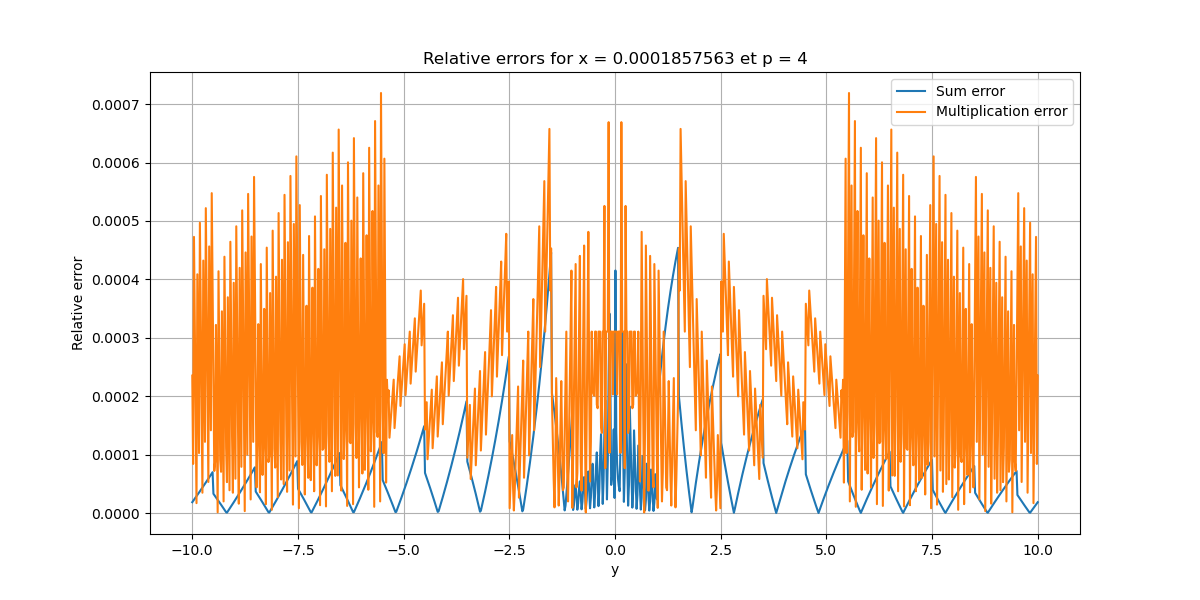
\includegraphics[width=\linewidth]{Figure_3.png}
        \caption{$x = 0.000185, p = 4$}
        \label{fig:erreur_x000185}
    \end{subfigure}
    \caption{Évolution de l'erreur relative pour différentes valeurs de $x$}
    \label{fig:erreur}
\end{figure}



\indent A partir des graphique, nous avons remarqué un motif pair et périodique pour la multiplication qui apparait toutes les puissances entières de dix. Nous considérons que cette régularité toute les puissances de dix dépend de la base utilisée pour représenter les nombres. L'erreur relative augmente à l'approche d'une puissance de dix puis diminue après le passage de la puissance.
Entre deux puissances de dix, l'erreur est minimale pour les nombres les plus élevés et l'erreur est plus importante lorsque la mantisse diminue. \\
\indent Pour l'addition, l'erreur est plus importante lorsque \texttt{y} est proche de \texttt{-x}, car cela provoque une annulation partielle. 

\section{Convergence et erreur de l'approximation de $\ln(2)$}
Nous illustrons la convergence de l'approximation de $\ln(2)$ pour différentes valeurs de $p$. 
Plus $p$ est grand, plus la convergence est rapide.

\subsection{Convergence de $\ln(2)$}
Les figures ci-dessous montrent l'évolution de $\ln(2)$ en fonction du nombre d'itérations :

\begin{figure}[H]
    \centering
    \begin{subfigure}{0.4\textwidth}
        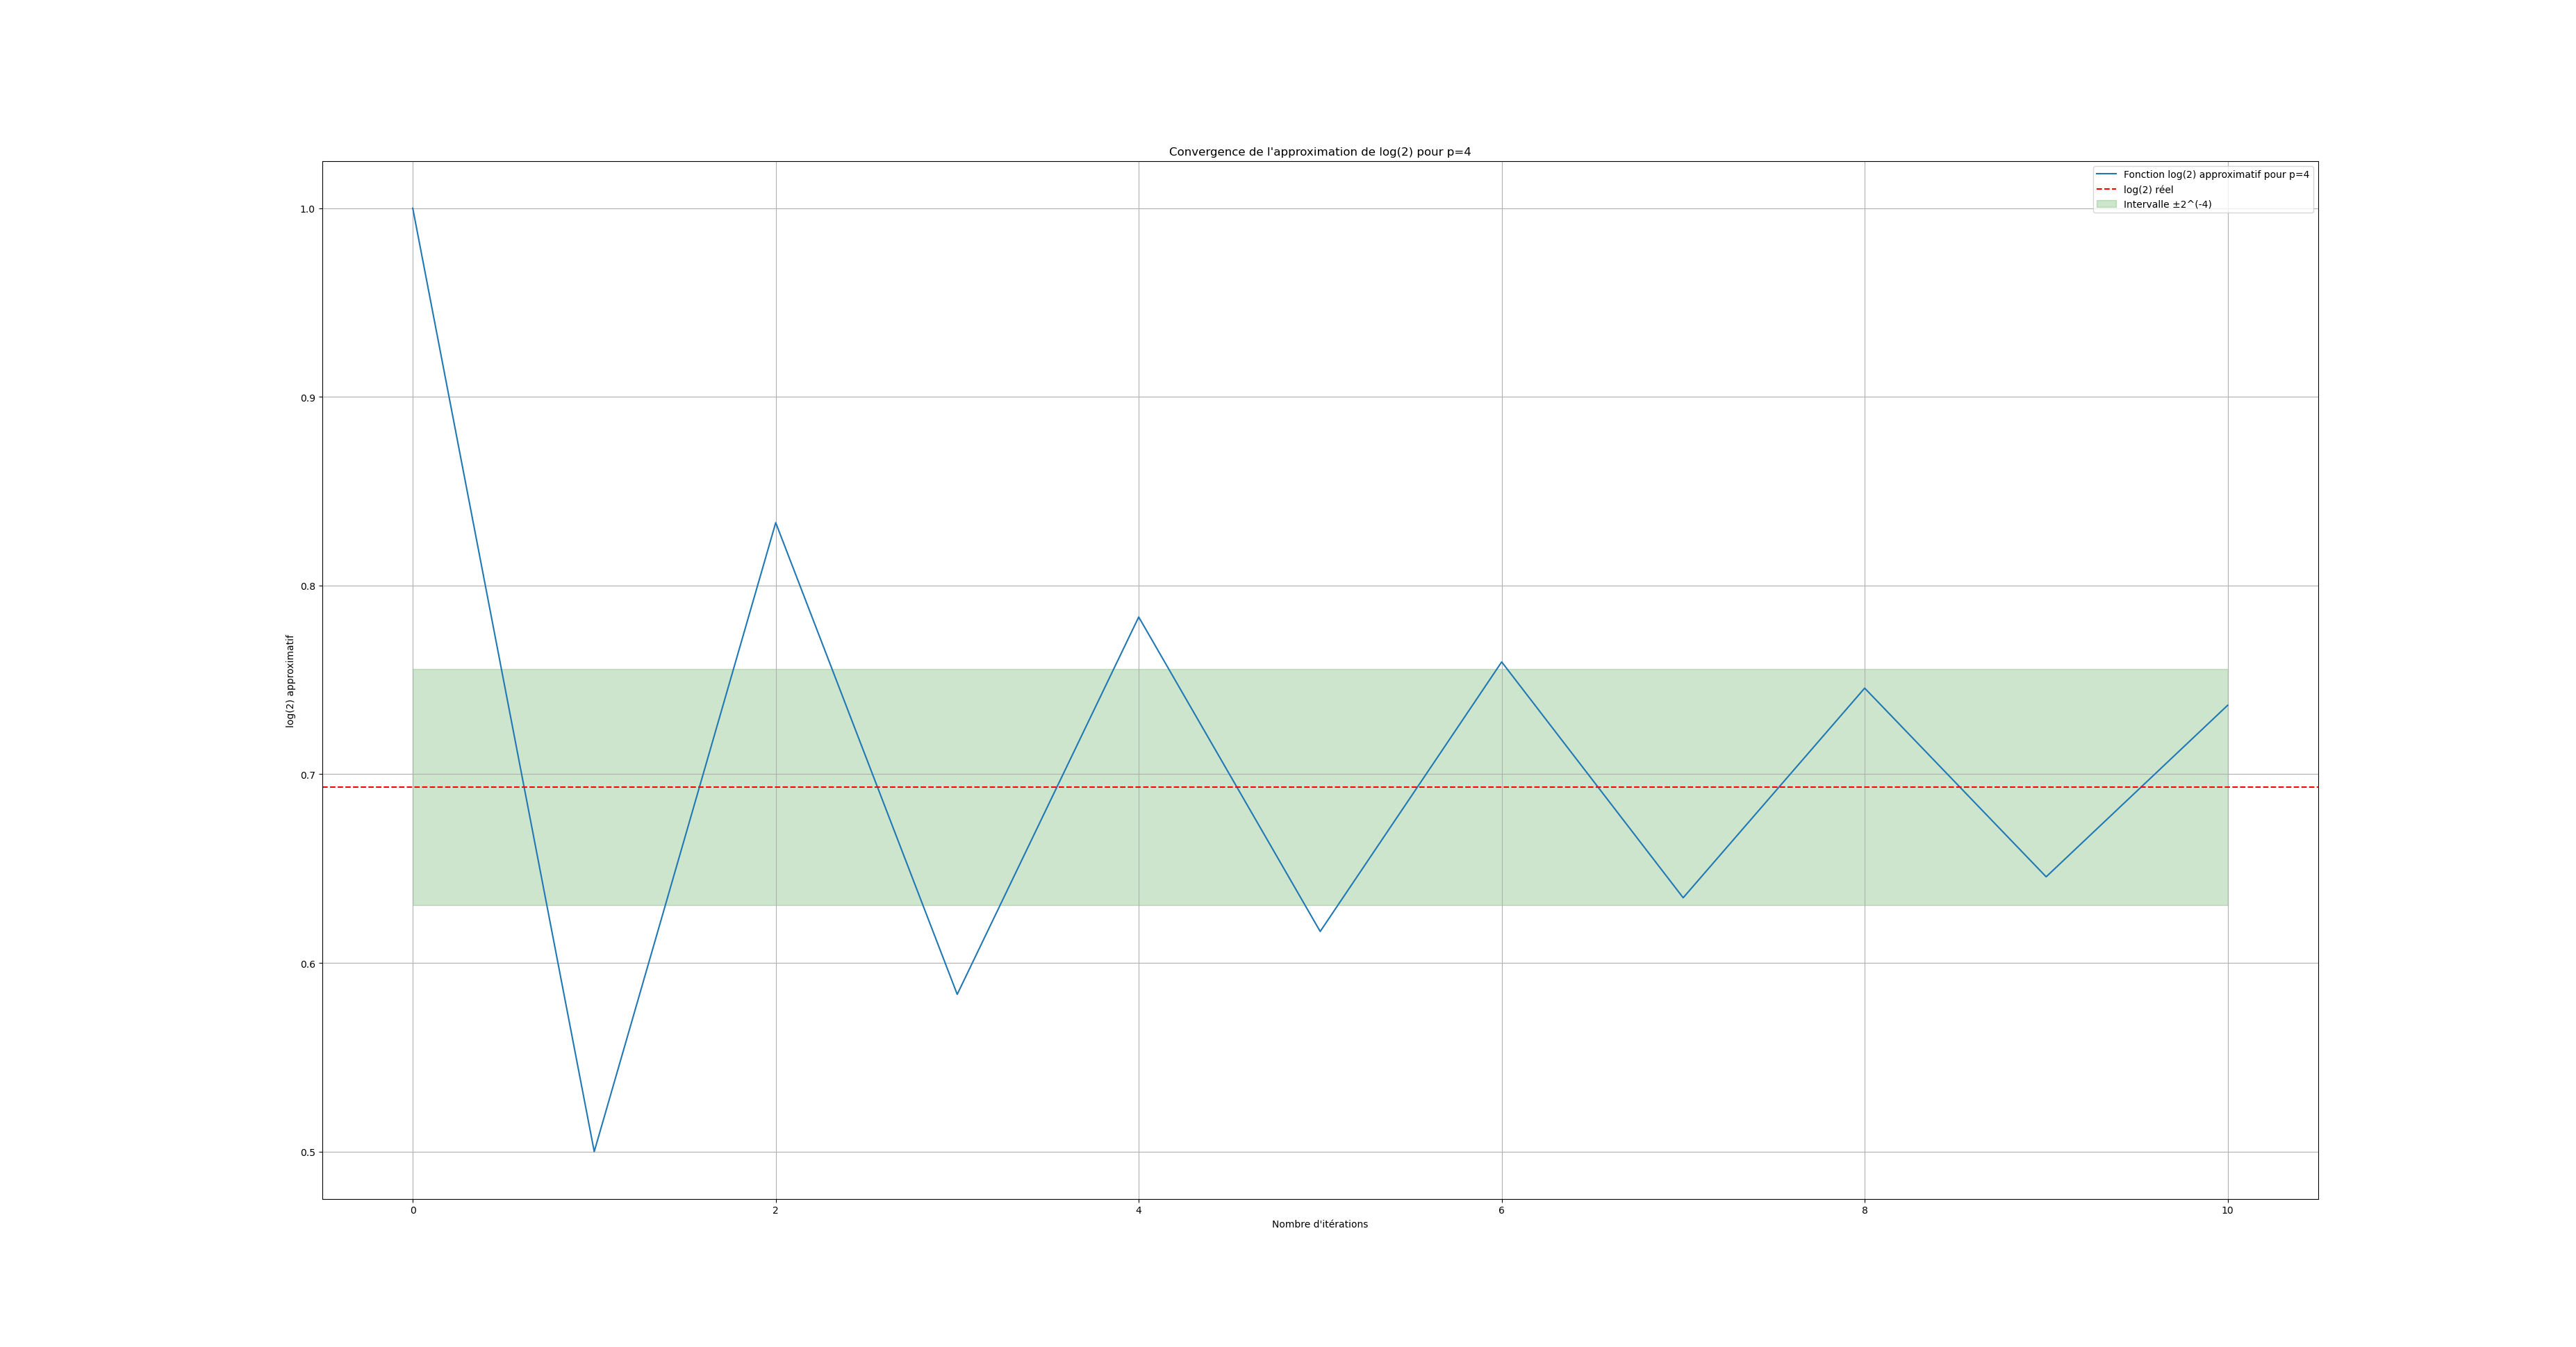
\includegraphics[width=\linewidth]{p=4.png}
        \caption{Convergence pour $p = 4$}
    \end{subfigure}%
    \begin{subfigure}{0.4\textwidth}
        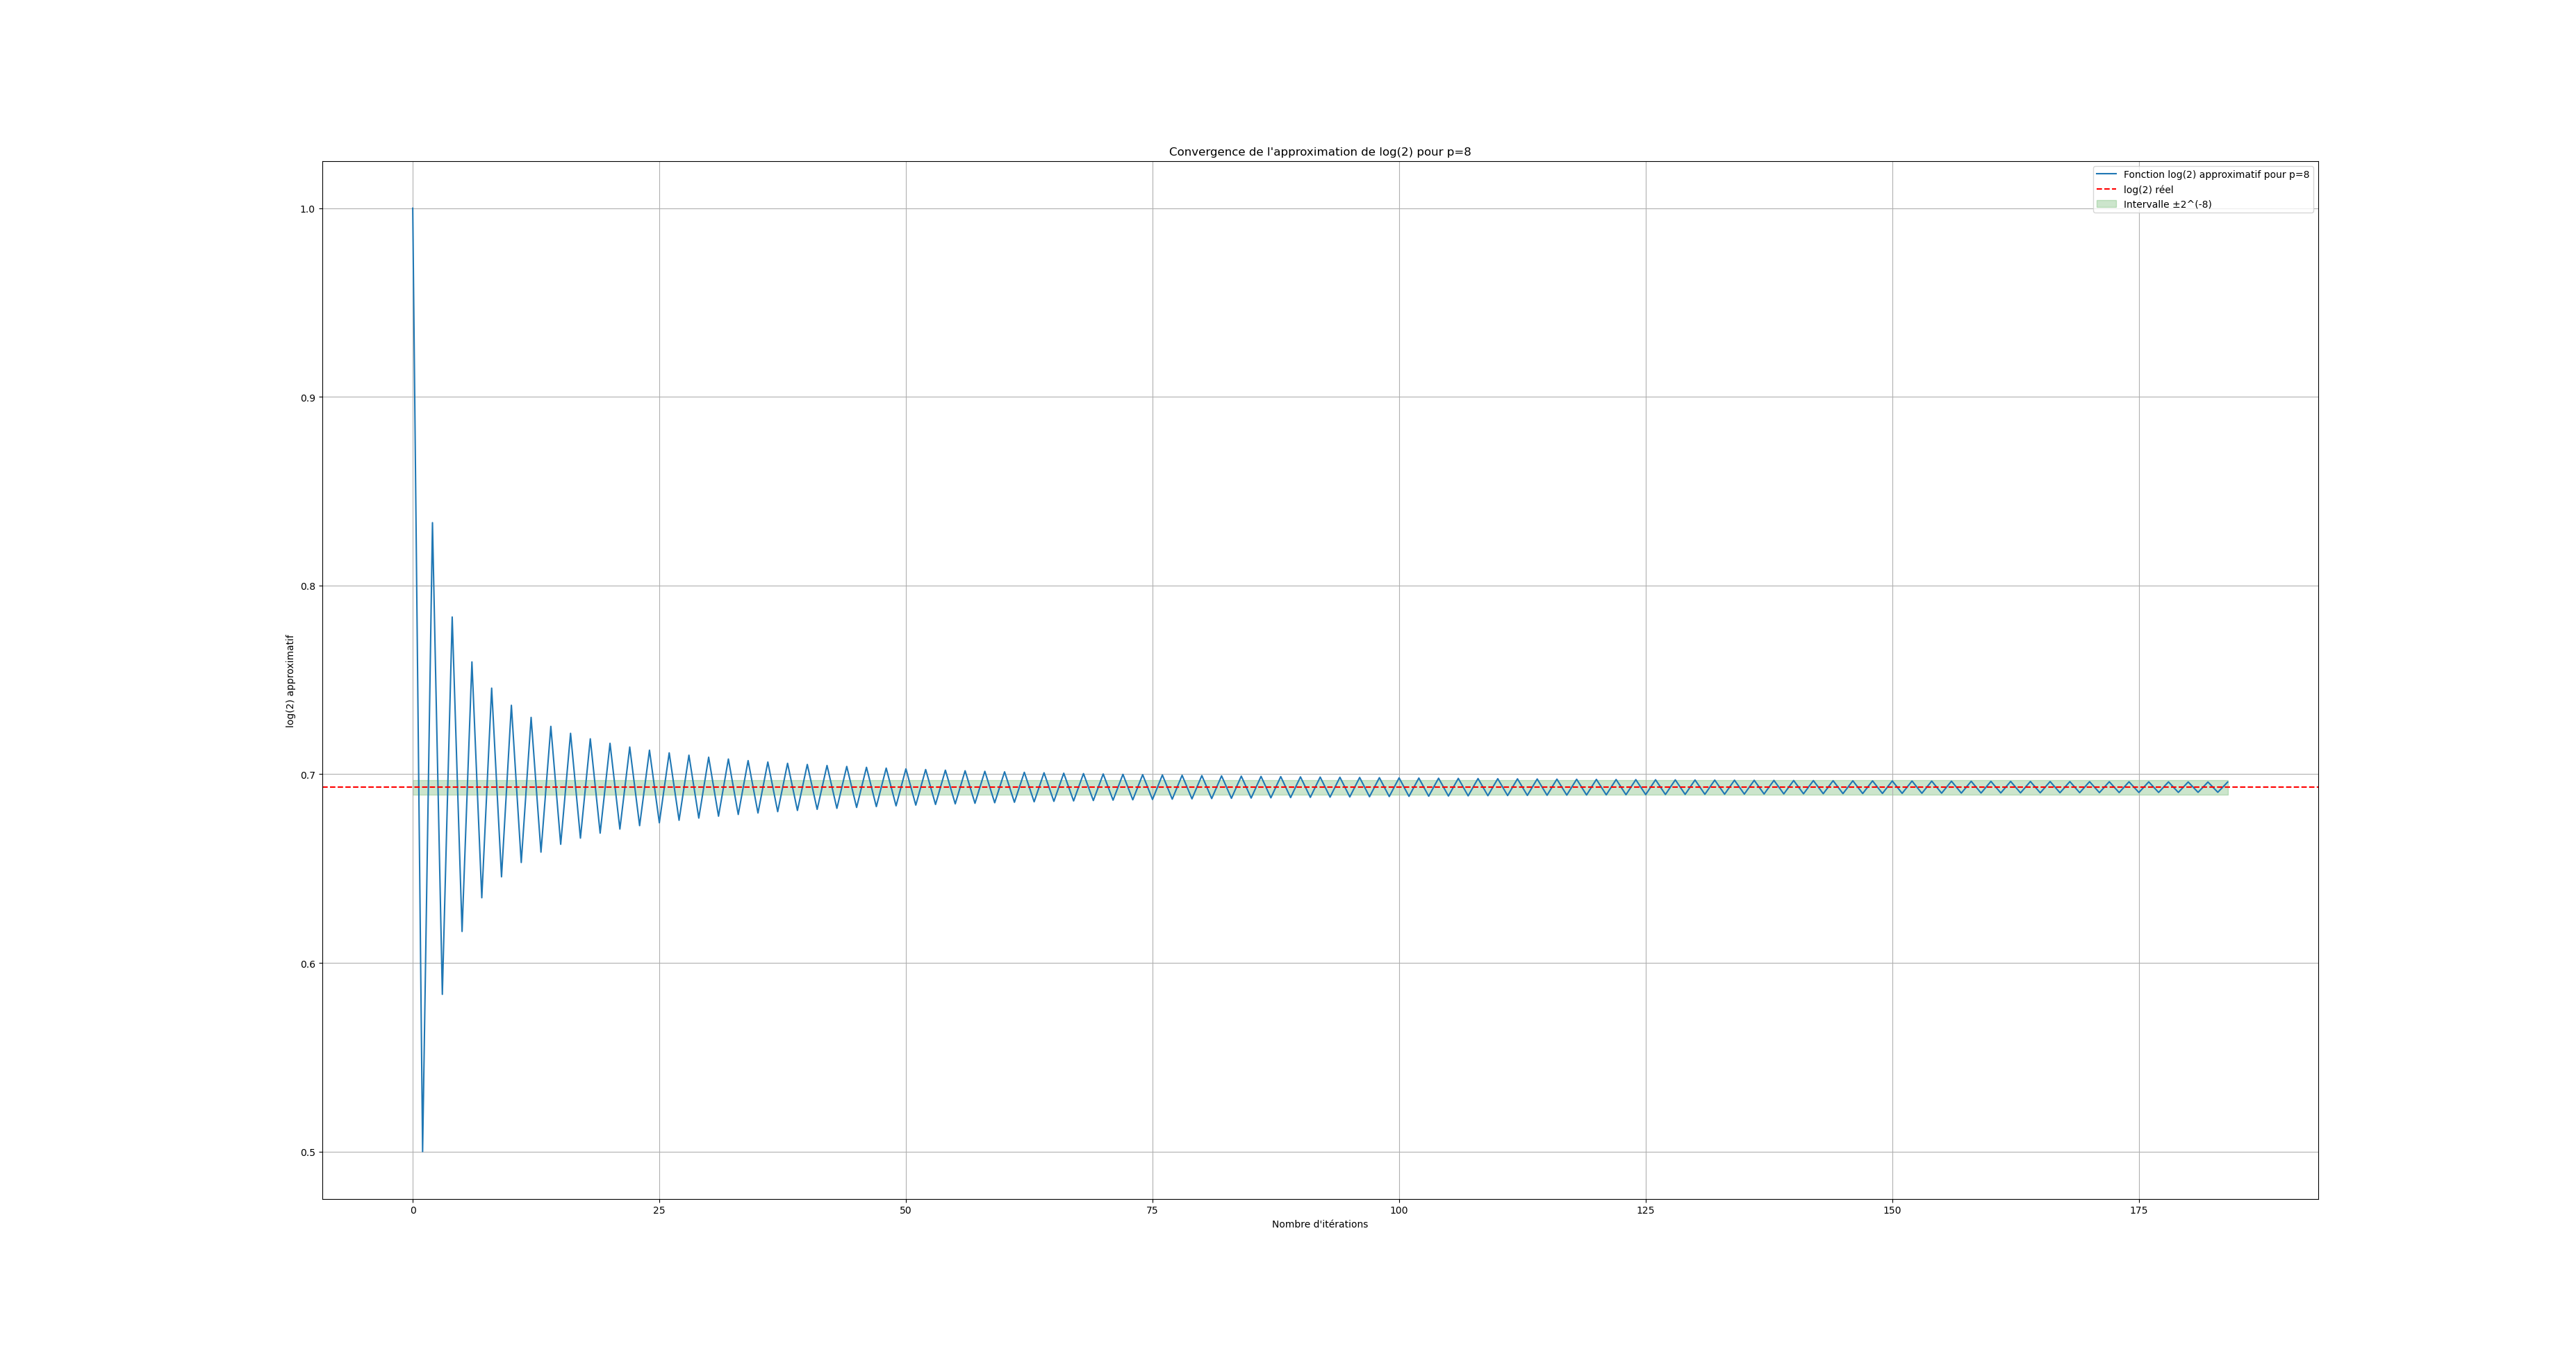
\includegraphics[width=\linewidth]{p8.png}
        \caption{Convergence pour $p = 8$}
    \end{subfigure}
    
    \caption{Illustration de la convergence de $\ln(2)$ pour différentes valeurs de $p$. Plus $p$ est grand, plus la convergence est rapide.}
    \label{fig:convergence_ln2}
\end{figure}

\subsection{Évolution de l'erreur}
Nous observons que l'erreur diminue plus rapidement en fonction du nombre d'itérations lorsque $p$ augmente :

\begin{figure}[h]
    \centering
    \begin{subfigure}{0.4\textwidth}
        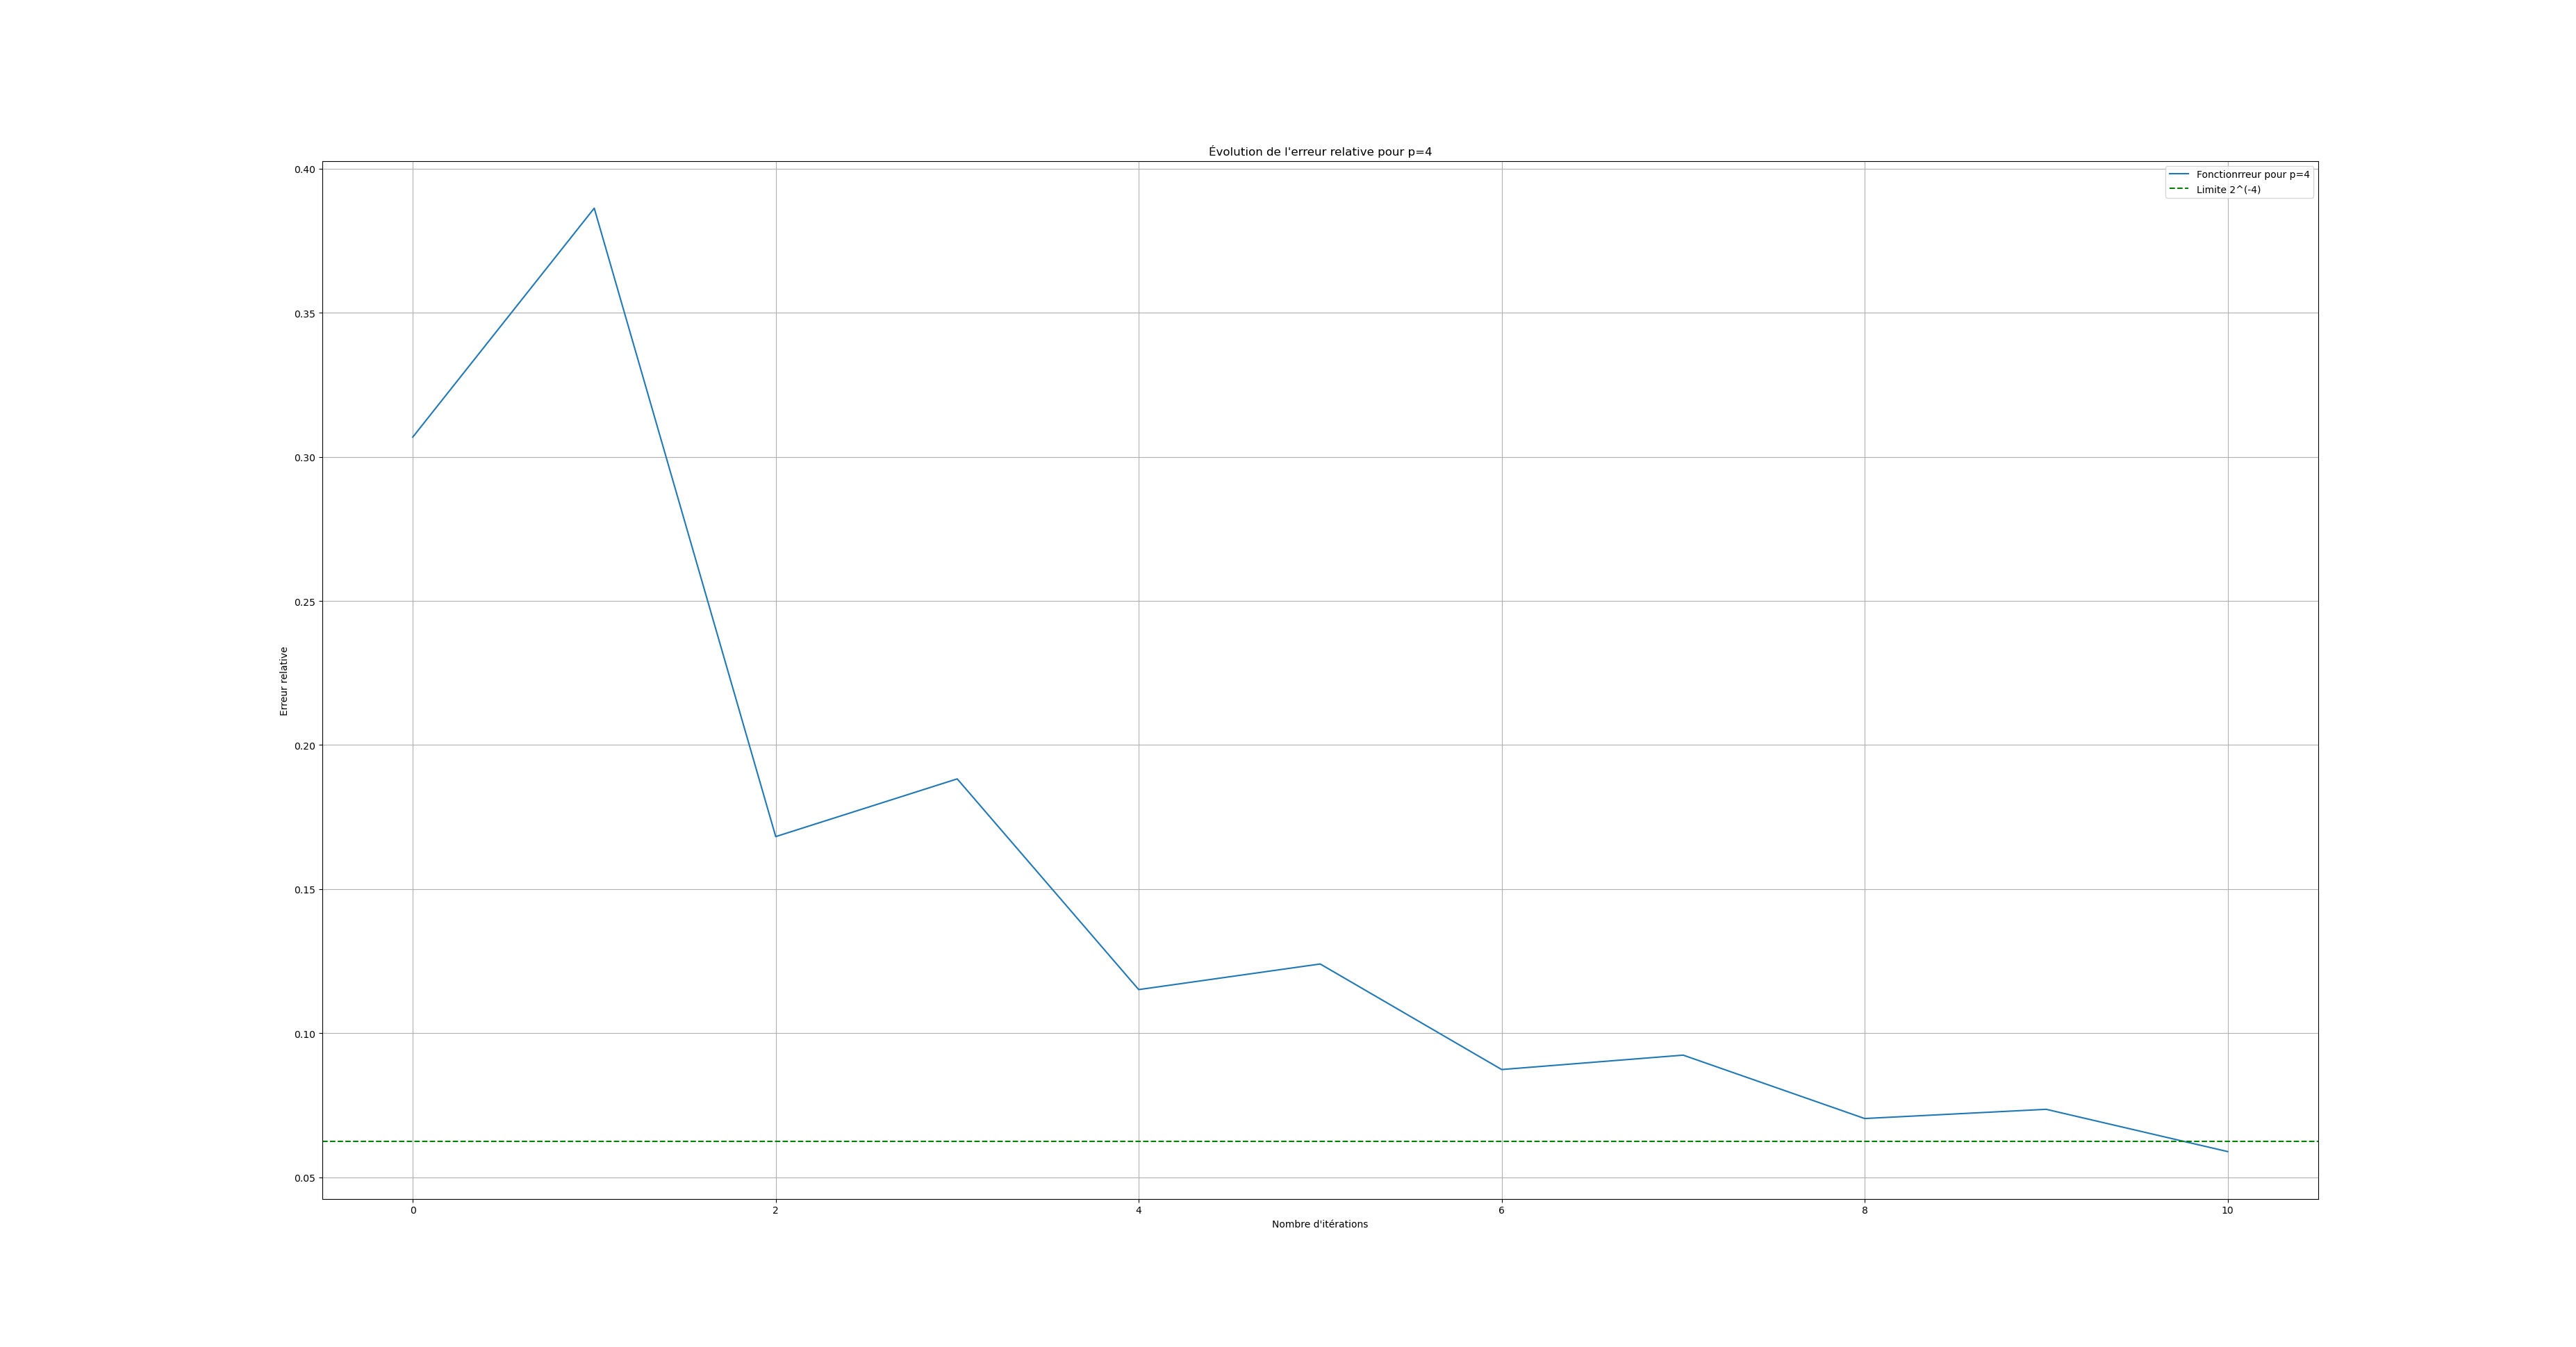
\includegraphics[width=\linewidth]{errp4.png}
        \caption{Erreur pour $p = 4$}
    \end{subfigure}%
    \begin{subfigure}{0.4\textwidth}
        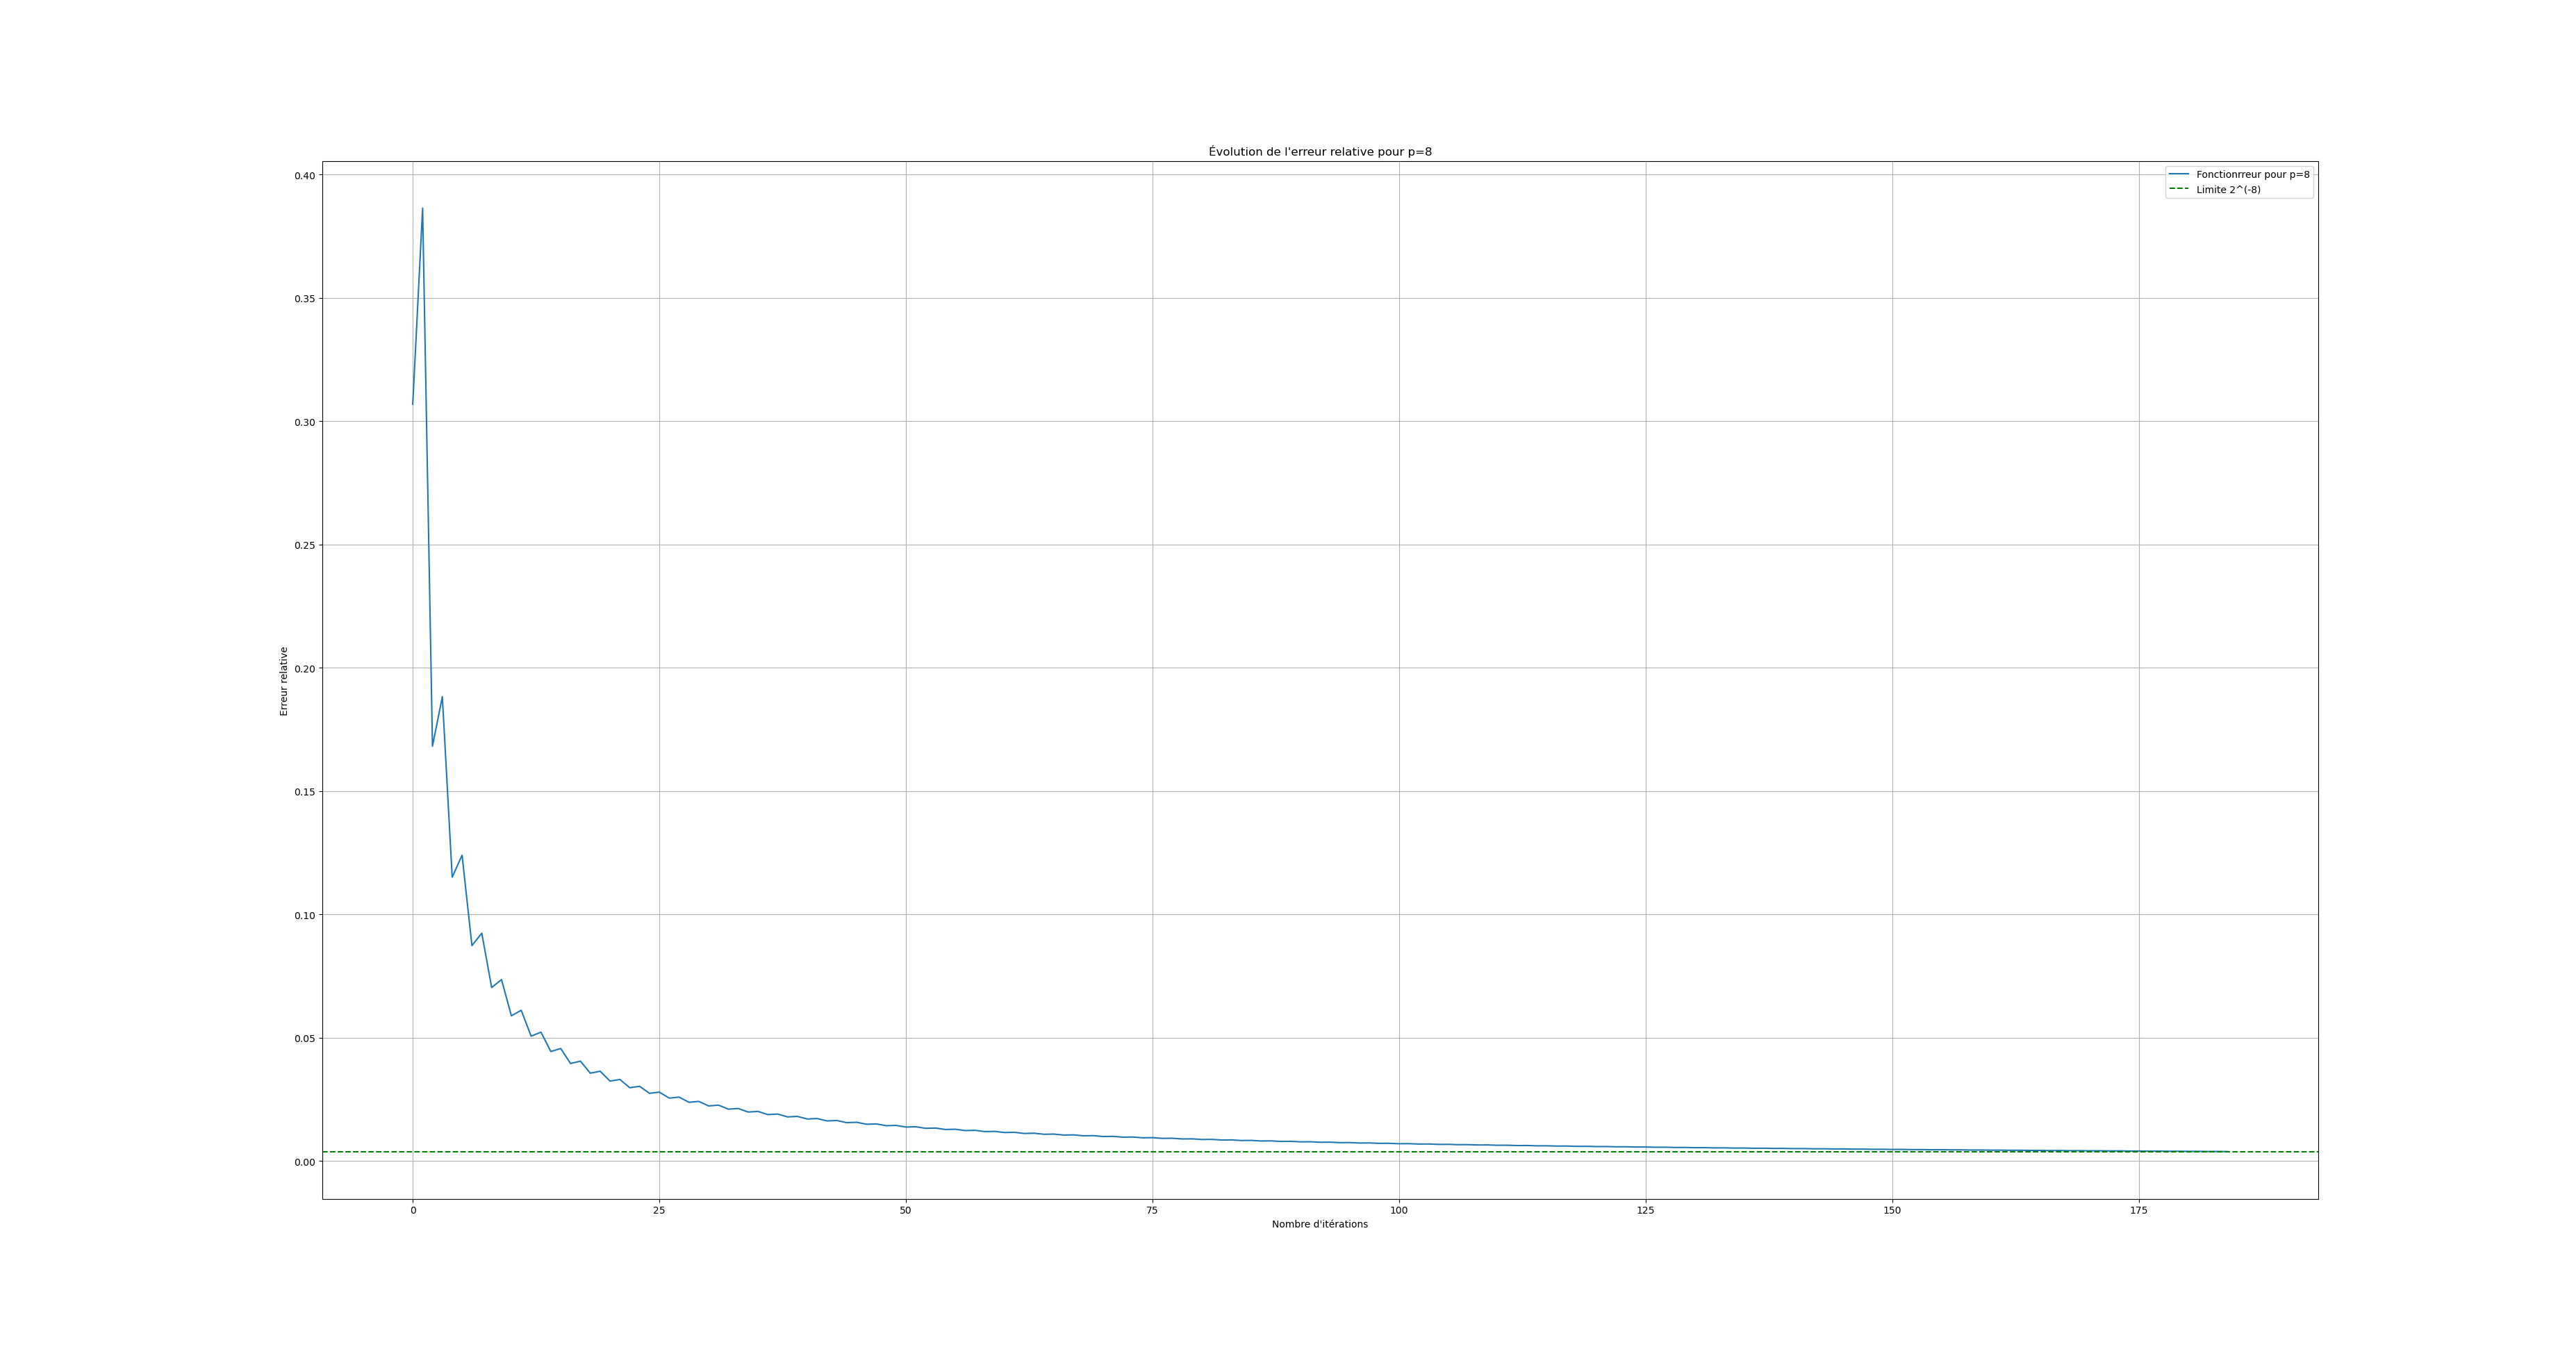
\includegraphics[width=\linewidth]{errp=8.png}
        \caption{Erreur pour $p = 8$}
    \end{subfigure}


    \caption{Évolution de l'erreur en fonction du nombre d'itérations pour différentes valeurs de $p$. On observe que l'erreur diminue plus rapidement lorsque $p$ augmente.}
    \label{fig:erreur_ln2}
\end{figure}

    

\section{Exemples d'algorithmes numériques}
\label{sec:algo_mun}
\subsection{Approximation de \texorpdfstring{$\log(2)$}{log(2)}}
Nous implémentons une méthode d'approximation de $\log(2)$ par la série alternée :
\begin{equation}
    \log(2) = \sum_{k=1}^{\infty} \frac{(-1)^{k+1}}{k}
\end{equation}
\begin{algorithm}
\caption{Approximation de $\log(2)$ par série alternée}
\begin{algorithmic}[1]
    \State $\log_{\text{réel}} \gets \log(2)$
    \State $\log_2 \gets 0$
    \State $n \gets 1$
    \While{True}
        \State $terme \gets \frac{(-1)^{n+1}}{n}$
        \State $\log_2 \gets \text{rp\_sum}(\log_2, \text{rp}(terme, p),p)$
        \State $\text{erreur} \gets \left| \frac{\log_{\text{réel}} - \log_2}{\log_2} \right|$
        \If{$\text{erreur} < 2^{-p}$}
            \State \textbf{Break}
        \EndIf
        \State $n \gets n + 1$
    \EndWhile
    \State \Return $\text{erreur}, \text{rp}(\log_2, p)$
\end{algorithmic}
\end{algorithm}

L'erreur est calculée à chaque itération, et nous arrêtons l'approximation lorsque l'erreur devient inférieure à $2^{-p}$.  

D'après la diapositive 23 intitulée \textit{"Erreur relative et précision machine"} des \textit{Slides du Projet 1} , l'erreur relative est bornée par :  

\begin{equation}
\frac{x - \text{rp}(x)}{x} \leq 2^{-p}
\end{equation}

où $\epsilon = 2^{-p}$ représente la précision machine. Ainsi, pour une précision machine simple, nous adoptons ce critère d'arrêt afin de garantir une approximation cohérente avec la limite de précision imposée par la représentation numérique.


\subsection{Représentation des nombres sur une calculatrice}

Les nombres sur une calculatrice sont représentés sur 8 octets en utilisant un format en \textit{Binary Coded Decimal} (BCD). Cette représentation se compose de plusieurs éléments :
\begin{itemize}
    \item Une \textbf{mantisse} constituée de 13 chiffres, chacun codé indépendamment sur 4 bits en BCD.
    \item Un \textbf{exposant}, qui est une puissance de 10, éventuellement signé.
    \item Un \textbf{signe} associé au nombre et, si nécessaire, à l’exposant.
\end{itemize}

\textbf{Ses avantages : } 
\begin{itemize}
    \item Une multiplication (ou division) par $10^n$ peut être remplacée par un simple décalage de $4n$ chiffres binaires, ce qui optimise certaines opérations arithmétiques.
    \item Sur calculatrice, on cherche à éviter les opérations lourdes comme la multiplication et la division, et le codage BCD permet de simplifier certains calculs en conservant une structure décimale.
\end{itemize}

\textbf{Ses inconvénients :  } 
\begin{itemize}
    \item Elle occupe plus d'espace mémoire, car chaque chiffre décimal est stocké sur 4 bits, alors qu'en binaire, on pourrait stocker plus d'informations sur le même nombre de bits.
    \item Elle peut entraîner des erreurs d’arrondi, particulièrement lors de soustractions entre des nombres proches ou lorsque plusieurs opérations comme des multiplications successives sont effectuées. Ces erreurs de précision peuvent s'accumuler et affecter les résultats finaux.
\end{itemize}


\subsection{Optimisation des calculs}
Les calculatrices utilisent principalement l'algorithme \textbf{CORDIC} pour calculer les fonctions trigonométriques et exponentielles. Cet algorithme repose sur un principe simple : il effectue une série de rotations successives en utilisant des additions et des décalages de bits, ce qui permet d'éviter des opérations plus complexes comme les divisions ou les multiplications classiques. Cette méthode est particulièrement adaptée aux calculatrices, car elle permet de réaliser les calculs rapidement et efficacement, tout en minimisant la consommation de ressources matérielles.

\subsection{Implémentation des Fonctions CORDIC}
Nous avons implémenté plusieurs fonctions mathématiques avec la méthode CORDIC :
\begin{itemize}
    \item \texttt{ln\_CORDIC(x)} pour le logarithme népérien
    \item \texttt{exp\_CORDIC(x)} pour l'exponentielle
    \item \texttt{arctan\_CORDIC(x)} pour l'arc-tangente
    \item \texttt{cordic\_tan(x)} pour la tangente

\end{itemize}

Ces algorithmes permettent d'approximer ces fonctions avec uniquement des additions, soustractions et décalages binaires, optimisant ainsi les calculs sur du matériel à ressources limitées.

\section{Conclusion}

Ce projet a mis en lumière les limitations de la représentation des nombres en machine et les erreurs numériques qui en découlent. Nous avons observé que :
\begin{itemize}
    \item L'erreur relative est influencée par la position des nombres par rapport aux puissances de dix ;
    \item Certaines opérations comme l'addition peuvent générer des erreurs importantes en cas d'annulation partielle ;
    \item L'analyse des erreurs est essentielle pour garantir la stabilité des algorithmes numériques.

\end{itemize}
Une meilleure gestion des erreurs peut être obtenue par des méthodes de calcul plus robustes, comme l'utilisation d'algorithmes adaptés ou l'augmentation de la précision des nombres flottants.\\
\indent Ce rapport met en évidence l'impact des erreurs numériques dans les opérations élémentaires et leur propagation dans les calculs avancés. L'utilisation de représentations en précision limitée impose des choix algorithmiques adaptés, comme la méthode CORDIC pour éviter les multiplications et divisions coûteuses. 
\end{document}